\chapter{FANET routing protocol}
Each multi-UAV mission has its own set of requirements in terms of size and number of vehicles, the size of the mission's region, payload, mission duration, environmental constraints, level of autonomy and mobility requirements. These all mission-oriented requirements - in turn - generate a peculiar set of demands from the communication infrastructure. Therefore, we will first present an overview of our multi-UAV mission at hand, the communication requirements and then a protocol that facilitates those primitives.

\section{FANET Mission}

The use of multi-cluster UAVs to track gas plumes like volcanic eruptions, forest fires, and environmental contamination has increased in the previous decade. The network requirement from a FANET depends on the mission. For example, in a plume tracking mission, the UAVs would be required to wrap around the plume, report the contamination level and possibly move with the plume. As the plume moves in time and space the UAVs need to plan their trajectories in cooperation with each other to evenly spread out on the surface of the plume while maintaining a safe distance from each other and avoiding any static or dynamic obstacle in their path. A detailed description of the problem and a multi-UAV distributed solution has been provided in \cite{8080382}. The initial formation of drones is shown in \fref{fig:mesh_formation}. As an aid to visualization think of the mesh as a piece of cloth moving towards a spherical ball and eventually wrapping around the ball. As shown in \fref{fig:mesh_formation} the UAVs start in the mesh formation and move towards the plume. Whenever a UAV detects a contamination it stops while rest of the UAVs continue their path. Eventually, the inter-UAV distance crosses a threshold and the moving drone tries to move closer to the stopped UAV. These inter-drone forces maintain an approximate mesh structure while resulting in the UAVs wrapping around the plume. A desired final state of UAVs wrapped around the plume is shown in \fref{fig:final_state}.  

\begin{figure}[hbtp]
\centering
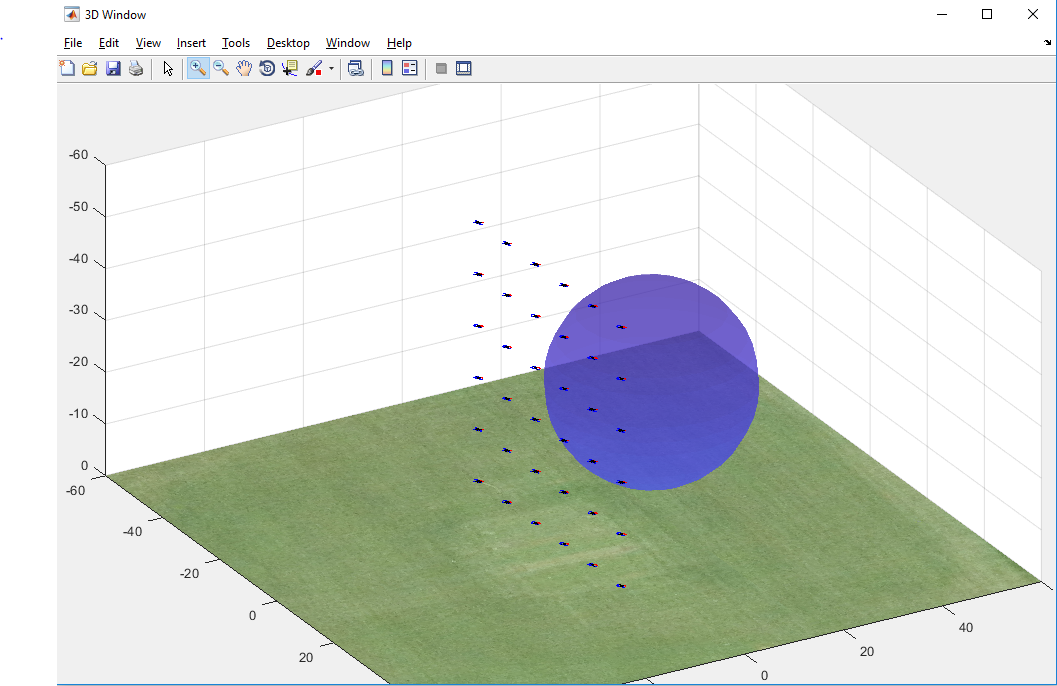
\includegraphics[width=0.8\textwidth]{Chapter-3/figs/initial_drone_config}
\caption{Mesh formation of UAVs at the start of the mission}
\label{fig:mesh_formation}
\end{figure}

\begin{figure}[hbtp]
\centering
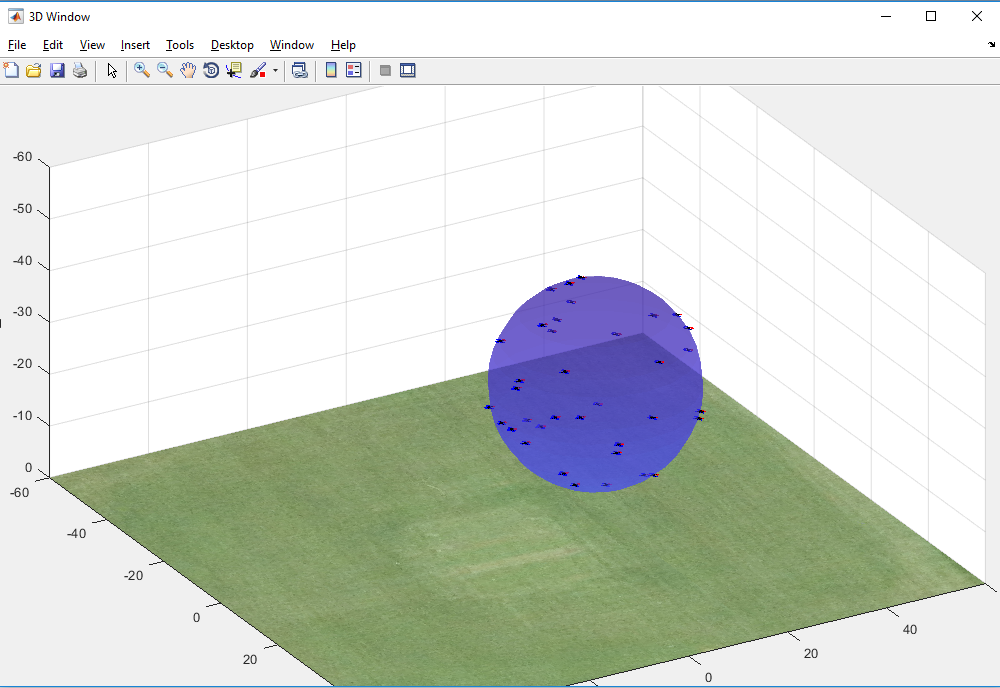
\includegraphics[width=0.8\textwidth]{Chapter-3/figs/final_formation}
\caption{Desired final state of UAVs wrapped around the plume}
\label{fig:final_state}
\end{figure}

Some of the assumptions made in \cite{8080382} are 
\begin{itemize}
\item{The shape of the plume is spherical, a simple convex hull.}
\item{When the mission starts the UAVs are arranged in a mesh formation moving towards the plume.}
\item{The UAVs have sensors which can detect the contamination after the density crosses a certain threshold.}
\item{All the UAVs are in direct radio range of each other}
\item{The location of each UAV is known at all time in an absolute 3D space}
\end{itemize}

In this work we relax the last two assumptions, i.e. all the UAVs are \emph{not} within the direct broadcast range and a UAV always knows its own location via GPS but \emph{doesn't know} the location of other UAVs. To facilitate multi-hop message passing we will need an efficient routing protocol which is a goal of this work.

\section{Communication requirements} \label{comm_reqs}
\textbf{Content}: There are different network requirements for communicating telemetry/ coordination and sensed data, some of them are delay tolerant and some need to be delivered to a specific region.

\textbf{Intent}: Discuss the scenarios where uav-to-uav, uav-to-ground station unicast would be required and the scenarios where geocast would be suitable. 

From a communications viewpoint, the UAVs need to communicate in different conditions which require specific message primitives. In this section, we shall discuss the specifics of such situations and the message primitives. Following are the communications requirements among the UAVs specific to the mission.
\begin{enumerate}
\item Since the UAVs are required to maintain an approximate mesh structure they need to approximate the distance with other drones. Therefore, the UAVs need to update each other of their GPS locations. This requires a facility to flood a message throughout the network. 

\item Sometimes, the UAVs need to navigate around each other while avoiding a collision. To check if the destination location (or the path) is void of other UAVs, the UAV sends a periodic beacon message to its destination geographic region. If some other UAV happens to be in the region then they negotiate their way around. It should be noted that the originator UAV doesn't know or care about the identity of the drone, rather the message is addressed to the geographical region. This requires a capability to geocast packets where the destination location is the address. These messages are \emph{not} delay-tolerant and need to be delivered in real time.
\item In some missions where the cluster is formed of UAVs of different capabilities (some UAVs have extra sensors), there would be a need of one-to-one communication between the UAVs in real-time. Even in other scenarios, there would be a need for one-to-one communication. This necessitates, a facility to send unicast messages to a specific destination UAV.
\end{enumerate}

In summary, we need to define and facilitate the following message primitives.
\begin{enumerate}
\item \emph{Flood(message, sourceUAV)}
\item \emph{Unicast(message, sourceUAV, destinationUAV)}
\item \emph{Geocast(message, sourceUAV, destinationCoordinates, radius)}
\end{enumerate}
Arguments like \emph{sourceUAV} and \emph{destinationUAV} are unique identifiers - possibly IP addresses, while \emph{destinationCoordinates} together with \emph{radius} represent a spherical region with specified coordinate as the center and specified radius.

\section{Routing protocol} \label{routing_protocol}

\textbf{Content: Discuss the location service employed to get destination location, packet header, message primitives and packet routing strategy.}

\textbf{Intent: Explain how a node knows the location of the destination node, and when a node transmits a received message.
}

In this section, we shall describe the mechanism and the parameters for the routing protocol as employed in the message primitives. 
These are our assumptions while designing the algorithm: 
\begin{enumerate}
\item The wireless antennas on the nodes are omnidirectional.
\item The nodes are reachable from each other i.e. a flooding algorithm can guarantee packet delivery between any pair of nodes and we use the delivery rate of flooding algorithm as an upper bound for our algorithm.
\item The nodes always know their location via GPS. 
\item A source node knows an approximate location of the destination node which is maintained in a location table and provided by a location service. Different implementations of a location service have been mentioned in section \ref{loc_service} and our implementation has been explained in section \ref{loc_service_impl}. 
\end{enumerate}

These are the expectations of a routing algorithm that would be suitable for our mission. 
\begin{enumerate}
\item Packet delivery rate between any two pairs of nodes should be approximately equal to a flooding algorithm. 
\item The average number of total transmission per transmitted packet should be significantly lower than flooding.
\end{enumerate}

\paragraph{Packet Header} \label{packet_header}
We first define the packet header that the source node attaches to the payload.
\begin{itemize}
\item Packet ID (\emph{pId}): A number that uniquely identifies this packet among those transmitted by this node. The combination of source node identification and packet ID should uniquely identify a packet in the FANET. 
\item Source Node ID (\emph{srcId}): A unique identifier for the source node. It could be IP address of the node.
\item Source Location (\emph{sLoc}): The GPS coordinate of the source node.
\item Destination Node ID (\emph{destId}): A unique identifier for the destination node. If a packet is destined to a geographical region, then this shall be set to the macro ANY. If a packet is to be flooded in the network, then this value should be set to the macro FLOOD. 
\item Destination Location (\emph{dLoc}): GPS coordinate of the destination as known to the source node. In case of flood packet, this would be set to NULL or be ignored. 
\item Radius (\emph{r}): In case of a geocast packet, the radius along with dLoc defines the destination spherical region for the packet.
\item Transmitter ID (\emph{trId}): A unique identifier for the latest transmitter of the packet.
\item Transmitter Location (\emph{trLoc}): GPS coordinate of the node that had last transmitted the packet.
\item Timestamp (\emph{timestamp}): The time when this packet was transmitted by the source.
\item Width (\emph{w}): The width of the transmission zone for the packet. Explained later in this section.
\item Hops To Live (\emph{HTL}): A node forwards a message only if HTL > 0 and reduces HTL by 1 before forwarding the packet. 
\item Acknowledgement Required (\emph{ackReq}): This flag denotes whether the source node is expecting an \emph{ack} reply.
\item Update Allowed (\emph{update}): This flag denotes whether an intermediate node can update the message headers. For example, if the intermediate node has a location update that is later than the message's \emph{timestamp}.

\end{itemize}

\paragraph{Transmission Zone:} Consider source node 'S' (at \emph{sLoc}) needs to send a message to a destination location \emph{dLoc}. The source node will first create a message (\emph{msg}) and defines a volume in the form of a spheroid with \emph{sLoc} and \emph{dLoc} as the two foci points and parameter 'w' as the minor-axis length. An intermediate node 'N' forwards this msg if and only if 'N' lies inside the spheroid defined by the msg parameters. This idea of constrained flooding is derived from the concept of the petal in \cite{6133499} and that of request zone in \cite{Ko:1998:LRM:288235.288252}. To increase reliability, the source node can increase the parameter transmission zone's width 'w'.

A sample depiction of transmission zone is depicted in \fref{fig:spheroid}.

\begin{figure}[hbtp]
\centering
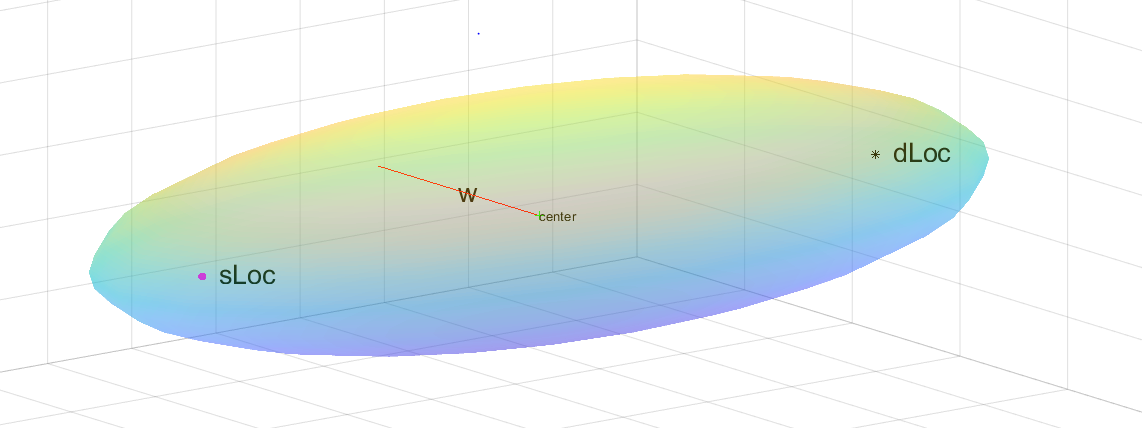
\includegraphics[width=1\textwidth]{Chapter-3/figs/Spheroid}
\caption{Transmission zone with source at sLoc and destination at dLoc}
\label{fig:spheroid}
\end{figure}

We now present a high-level algorithmic description of the message primitives described in section \ref{comm_reqs}.

\textbf{Flooding}
When a source node 'S' needs to send a message to every node in the network it creates a header with the following parameters.

\begin{eqnarray*}
header = & messageHeader(destId = FLOOD, dLoc = IGNORE, \\
    & radius = IGNORE, pdate = IGNORE, width = IGNORE, \\
    & ackReq = FALSE, HTL = NETWORK\textunderscore DIAMETER)
\end{eqnarray*} 

Source node `S' then encapsulates the data in this header. NETWORK\textunderscore DIAMETER is a macro which represents the maximum hops that a packet can travel. 

Node S then broadcasts this message in the wireless medium. An intermediate node 'N', on receiving the message for the first time reads the contents and rebroadcasts it. Afterward 'N' discards any duplicate receptions of the message. This guarantees that the flooding is loop-free.
The path of receive algorithm that deals with FLOOD packets is depicted in algorithm \ref{flood_recv}


\begin{algorithm}
\caption{Receive(msg): Flood} 
\label{flood_recv}
\DontPrintSemicolon
\SetKwProg{Flood}{Flood}{}{}
\Flood{(msg)}{%
    \eIf {msg.destId == FLOOD}{
        \eIf{msg.pId $\notin$ seenIdSet} {
            msg.HTL = msg.HTL - 1\;
            Add (seenIdSet, msg.pId)\;
            \If {msg.HTL > 0}{
                transmit(msg)\;
            }
        }{
            discard(msg)\;
        }
    }{
    ...
    }
}

\end{algorithm}


\textbf{Geocast}


When a source node 'S' needs to send a message to \emph{any} node in a spherical region 'R' with center at \emph{'dLoc'} and radius \emph{'r'} it chooses an appropriate width 'w' and creates a header with the following parameters.
\begin{eqnarray*}
header = & messageHeader(destId = ANY, dLoc = [x,y,z], radius = r,\\
    & update = IGNORE, width = w, ackReq = FALSE)
\end{eqnarray*}
Source node `S' then encapsulates the data in this header and transmits the packet.

\begin{algorithm}
\SetAlgoLined
\DontPrintSemicolon
\If{msg.pId is in transmittedMsgIdSet}{
    discard(msg)\;
    EXIT\;
}
\If{msg.destId == ANY}{
    \If{insideDestinationRegion(msg, myLoc)}{
        Transmit(msg)\;
        Add msg.pId to transmittedMsgIdSet\;
        EXIT\;
    }
}

\If{insideTransmissionZone(msg, myLoc) == TRUE}{
    \eIf{msg.pId is in bufWait}{
        Increase duplicate count for msg.pId\; 
        save msg.tLoc\;
    }{
        boffTime = calculateBoffTime(msg)\;
        add msg to bufWait \;
        
        registerCallback(boffTime, msg)\;
    }
}

\caption{Receive(msg): Geocast} \label{geocast_recv}
\end{algorithm}

\textbf{Unicast}

When a source node 's' needs to send a message to destination node 'D' then 'S' first consults its location table for the location of destination 'D' and creates a header with the following parameters.

\begin{eqnarray*}
header = & messageHeader(destId = destID, dLoc = [x,y,z], radius = IGNORE,\\
    & update = IGNORE, width = w, ackReq = FALSE)
\end{eqnarray*}

Source node `S' then encapsulates the data in this header and transmits the packet.

On the receiving side the node 'N' follows the following algorithm.

\begin{algorithm}
\SetAlgoLined
{...\;}
\eIf{msg.destId = myId}{
    \If{msg.ackReq == TRUE}{
        ackRep = prepareAckReply()\;
        send(ackRep);
    } 
}{
...
}
\caption{Receive: Unicast} \label{unicast_recv}
\end{algorithm}

\paragraph{Discussion - ROUGH}

Our routing algorithm doesn't maintain or exchange any topology graph hence it neither needs to exchange control information nor it has to do the computation heavy path calculations.

Moreover, our algorithm doesn't do a route discovery, which eliminates the typical delay associated with reactive routing algorithms. 

Our algorithm is robust i.e. the messages are routed through geo-diffuse pathsets and matches the delivery rate of flooding.